\documentclass[11pt,a4paper]{kth-mag}

% \usepackage{fontspec}
\usepackage[backend=bibtex]{biblatex}
% \usepackage[top=1cm]{geometry}
\usepackage{subfig}
\usepackage{graphicx}
\usepackage{hyperref}
\usepackage{moreverb}
% \defaultfontfeatures{Mapping=tex-text}
% \setromanfont[Ligatures={Common},Numbers={Lining}]{Linux Libertine}

\bibliography{report.bib}

\author{Michal Staniaszek}
\title{A Comparative Study on the Effect of Interest Point Methods and
  Descriptors on Feature-Feature Matching for Object Query in Point Clouds}

\begin{document}
\maketitle
\begin{abstract}
  Brief description of the aim of the project, the data used, some of the
  techniques used, some experimental results.
\end{abstract}
\tableofcontents
\chapter{Introduction}
Basic introduction to the idea of point clouds and how they are useful, as well
as something about images and querying them

In chapter~\ref{chap:bg}, we explain some concepts that are important to
understand the work, provide background information on relevant parts of the
image processing literature, and attempt to introduce the reader to previous
work in similar areas. The specific techniques used in our system are described
in chapter~\ref{chap:devel}, and we also discuss our reasoning behind certain
steps of the process. Chapter~\ref{chap:impl} deals with the software, and how
the system was implemented, along with some explanation of how the system
works. Our experimental setup and the results of the experiments are described
in chapter~\ref{chap:exp}. We compare the quality of retrieval when different
methods are used, and also investigate the time taken by the system under
varying conditions. Finally, we summarise the system and our results in chapter~\ref{chap:conc}.
\chapter{Background}
\label{chap:bg}
In this chapter we will introduce some key ideas relating to the project. While
some of the techniques described here are not directly used in the
implementation of our system, they can be useful for context, or to give
examples of different ways of approaching a similar problem. We discuss methods
of finding interesting regions in image and point cloud data, and how these
regions can be represented using descriptors.
\section{Segmentation}
Popularised by Comaniciu~\cite{comaniciu2002mean} for use in image segmentation,
mean shift was first introduced by Fukunaga~\cite{fukunaga1975estimation} in
1975, and rediscovered by Cheng~\cite{cheng1995mean} in 1995. The technique finds
stationary points in a density estimate of the feature space, for example pixel
RGB values, and uses those points to define regions in the space by allocating
pixels to them. Pixels which follow the gradient of the density to the same
stationary point are part of the same segment. An example can be seen in
Figure~\ref{fig:meanshift}.
\begin{figure}[t]
  \centering
  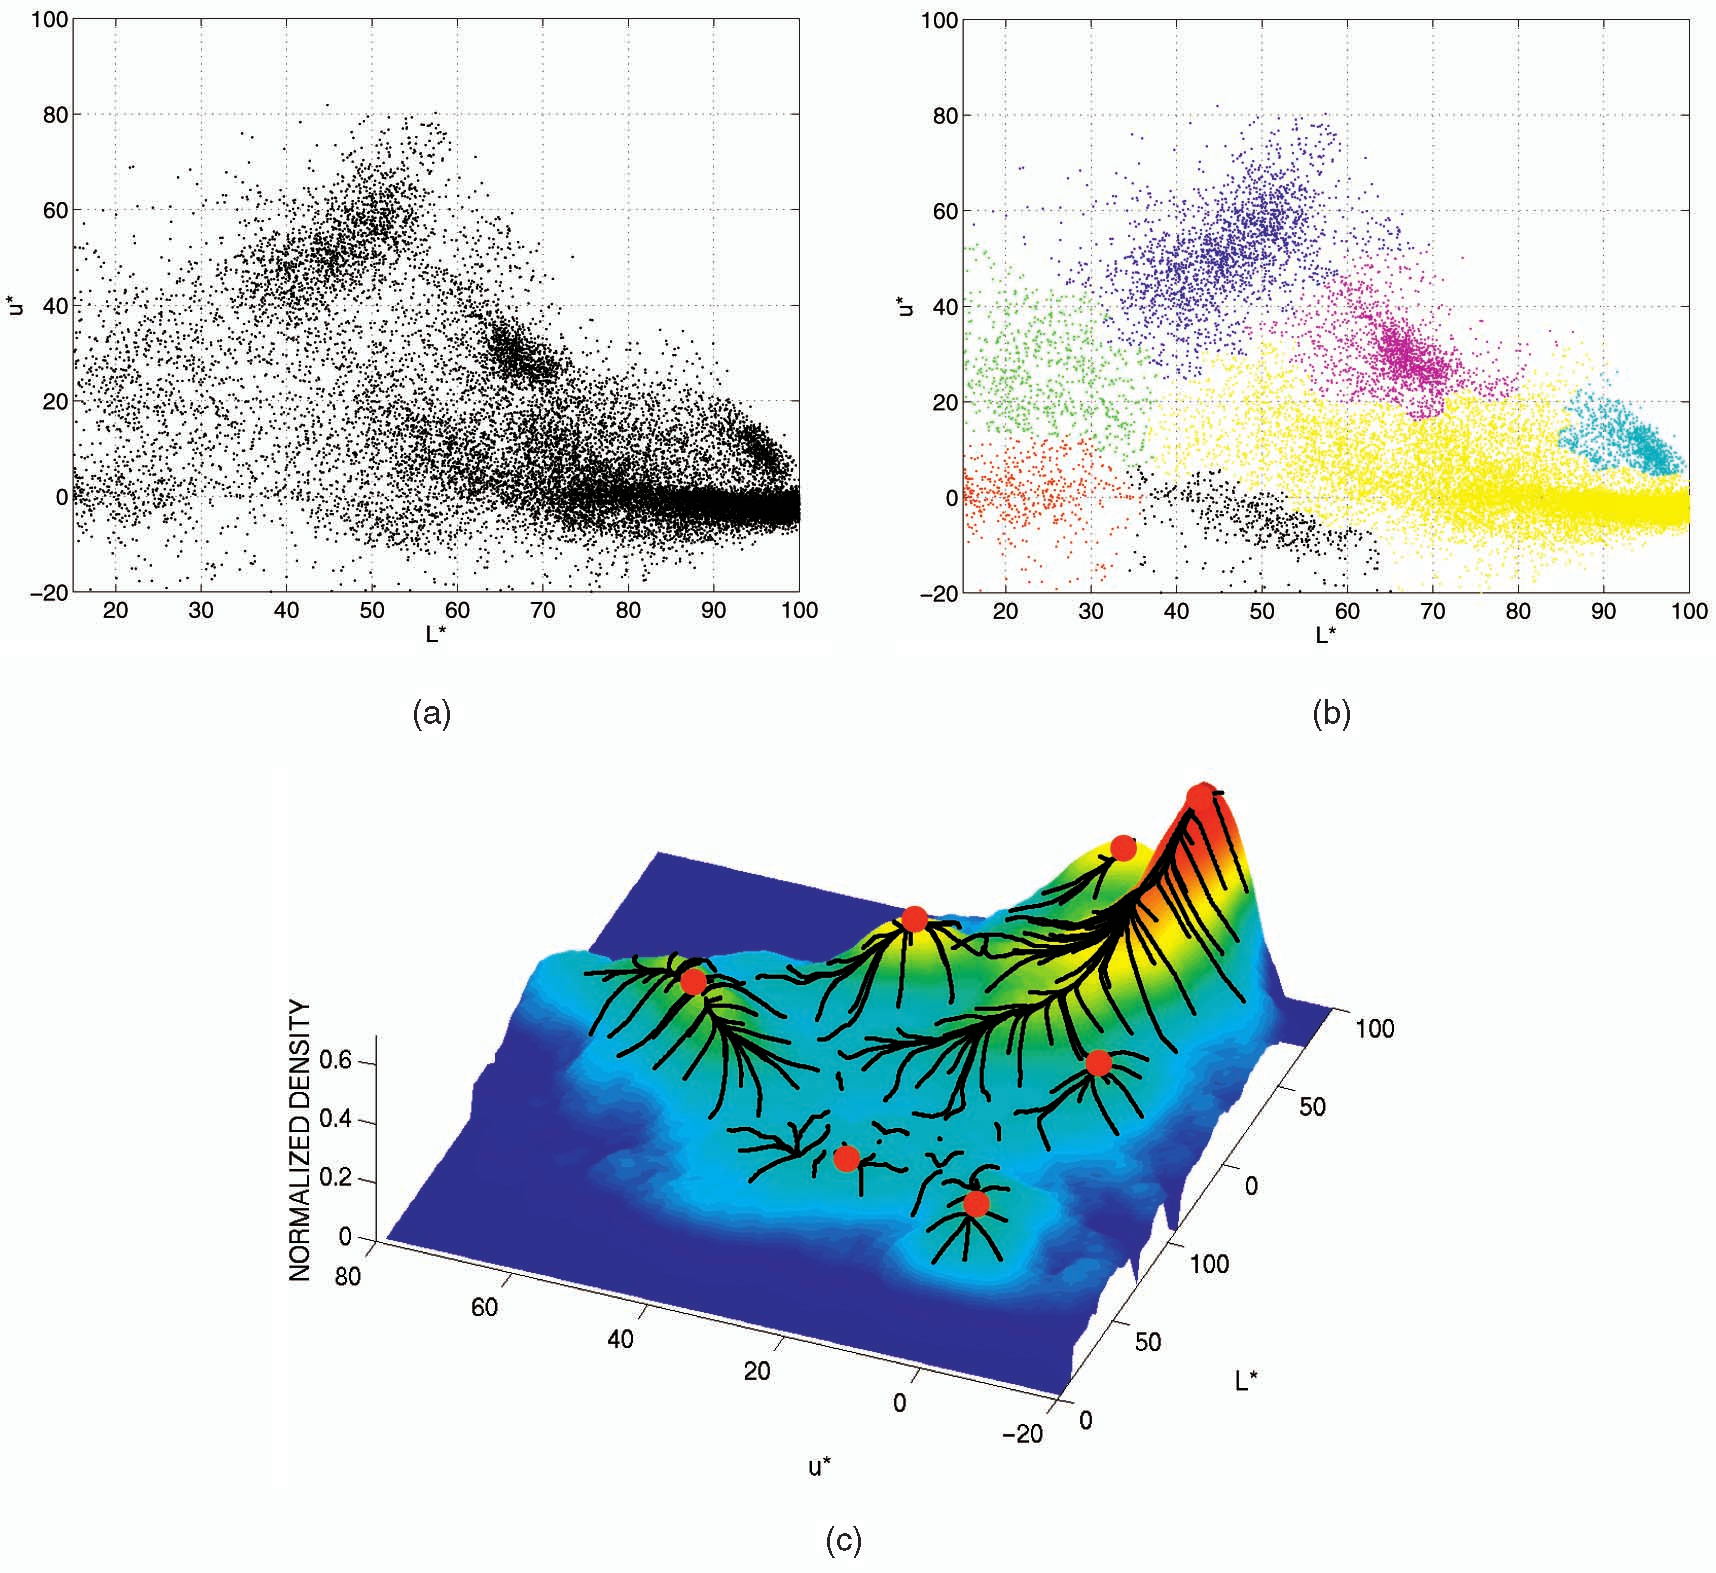
\includegraphics[width=\textwidth]{images/meanshift}
  \caption{Visualisation of mean shift \cite{comaniciu2002mean}. a) First two
    components of image pixels in LUV space. b) Decomposition found by running
    mean shift. c) Trajectories of mean shift over the density estimate.}
  \label{fig:meanshift}
\end{figure}

Random Sample Consensus (RANSAC) is a technique which uses shape models to find
ideal models in noisy data. Points in the data set are randomly sampled, and
used to construct a shape. For example, in the case of a line, two points are
sampled, and define the line. Distances from points in the data set to the model
defined by the randomly sampled points are then computed to find points which
are inliers to the model. This number is stored, and the process repeated a
number of times. At the end of the process, the model with the largest number of
inliers is returned \cite{fischler1981random}. RANSAC can be applied to
segmentation tasks by using it to find planes, cylinders, spheres and so on in
point clouds. In the case of planes this is particularly useful, as they are
usually not part of objects of interest, mostly making up walls, floors or
surfaces on which interesting objects rest. By removing the points corresponding
to these uninteresting surfaces, segmentation should be made easier. Several
extensions to RANSAC have been proposed. Maximum Likelihood Estimation Sample
Consensus (MLESAC) chooses a solution that maximises the likelihood of the model
instead of just the number of inliers \cite{torr2000mlesac}. M-estimator Sample
Consensus (MSAC) uses a different cost function to the original implementation,
additionally scoring the inliers depending on how well they fit the data
\cite{torr2000mlesac}. The Progressive Sample Consensus (PROSAC) uses prior
information about the likelihood of input data being an inlier or an outlier to
limit the sampling pool and greatly reduce computation cost
\cite{chum2005matching}.


\section{Methods for 2D}
While we are not directly interested in 2D descriptors, it may be instructive to
look at the techniques used in the selection of interest points and the way that
descriptors are constructed.
\subsection{Descriptors}
Van Gool \cite{van1996affine} gives a description of how to use moment
invariants to recognise planar patterns like labels and signs under affine
deformations. The moments describe things like the size of the shape and its centre
of mass, or statistics like the mean and variance of pixel intensities in the
shape. These moments can be combined in such a way that they are invariant to
deformations, which is useful to have in a descriptor.

\subsection{Combined Interest Point Extraction and Descriptors}
The Laplacian of Gaussians was introduced by Lindeberg, and uses derivatives
combined with some other techniques to select interest points.
\cite{lindeberg1998feature}. This paper also introduces the concept of automatic
scale selection for feature detection, which has played an important part in the
field since then. The scale of features can be investigated by blurring an image
using a Gaussian kernel --- higher standard deviation blurs the image more,
resulting in the removal of small scale features.

Even today the Scale Invariant Feature Transform (SIFT) is among the most
popular descriptors for 2D images. It is invariant to scale and rotation, and is
robust to some variation in affine distortion, viewpoint and illumination, and
is distinctive, allowing for correct matching of single features in large
databases. There are several stages of computation. Extrema are found in
different scales to find points invariant to scale and orientation. Keypoints
are selected at the extrema based on their stability. Image gradients at the
keypoint are used to define its orientation for future computations. The image
gradients are then transformed into a local descriptor vector with length 128
\cite{lowe2004distinctive}.

Mikolajczyk and Schmid~\cite{mikolajczyk2004scale} introduce the Harris-Laplace
detector which is an improvement on SIFT \cite{lowe2004distinctive} and the
Laplacian of Gaussians \cite{lindeberg1998feature} in the sense that it is able
to deal with affine transformations. They do not, however, introduce a new type
of descriptor to go with the point selection. 

Speeded-Up Robust Features (SURF) is a more recent descriptor which can be
computed and compared much faster than most other descriptors. It makes use of
integral images, which replace pixels in an image or image patch with a
cumulative sum of the pixel intensities over the rows and columns. This allows
for fast computation of pixel intensities in an area of the image. SURF takes
some ideas from SIFT, using the spatial distribution of gradients as a
descriptor, but integrates over the gradients instead of using individual
values, which makes it more robust to noise. The resulting descriptor is a 64
element vector, which means that it is also faster to compare than SIFT
\cite{bay2008speeded}.

\section{Methods for 3D}
\subsection{Interest Points and Saliency}
Sipiran and Bustos extend the popular Harris detector \cite{harris1988combined}
to 3D \cite{sipiran2011harris}. Knopp et al. extend the SURF detector to 3D
\cite{knopp2010hough}.

Shilane and Funkhouser introduce a distinctiveness measure over classes of
meshed objects \cite{shilane2007distinctive}.

A multi-scale signature defined by the heat diffusion properties of an object
called the Heat Kernel Signature (HKS) \cite{sun2009concise} is used in
\cite{ovsjanikov2009shape} to retrieve shapes.

\subsection{Descriptors}
One early descriptor which remains popular is the spin image. The descriptor is
generated from a mesh model at oriented points with a surface normal. A plane
intersecting the normal with a certain width and height is rotated around the
normal, forming a cylinder. The plane is separated into bins. The bins
accumulate the number of points which pass through a certain bin during the
rotation. The resulting 2D image is the descriptor. By varying the width of the
plane the region which defines the descriptor can be modified. A small width
will give a local descriptor, while a large width will give a descriptor for the
whole image \cite{johnson1997spin,johnson1999using}. Figure~\ref{fig:spinimg}
shows a visualisation of how the image is generated.

\begin{figure}
  \centering
  \subfloat{
    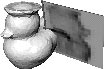
\includegraphics[width=0.11\textwidth]{images/spin1}
  }
  \subfloat{
    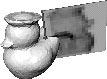
\includegraphics[width=0.11\textwidth]{images/spin2}
  }
  \subfloat{
    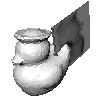
\includegraphics[width=0.11\textwidth]{images/spin3}
  }
  \subfloat{
    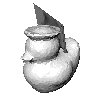
\includegraphics[width=0.11\textwidth]{images/spin4}
  }
  \subfloat{
    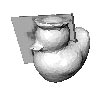
\includegraphics[width=0.11\textwidth]{images/spin5}
  }
  \subfloat{
    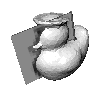
\includegraphics[width=0.11\textwidth]{images/spin6}
  }
  \subfloat{
    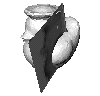
\includegraphics[width=0.11\textwidth]{images/spin7}
  }
  \subfloat{
    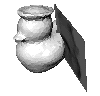
\includegraphics[width=0.11\textwidth]{images/spin8}
  }
  \caption{Frames from construction of a spin image \cite{johnson1997spin}. The
    image plane spins around the oriented point normal and accumulates points.}
  \label{fig:spinimg}
\end{figure}

The Ensemble of Shape Functions (ESF) descriptor introduced in
\cite{wohlkinger2011ensemble} by Wohlkinger and Vincze combines the Shape
Distribution approach introduced by \cite{osada2002shape} along with some
extensions proposed in \cite{ip2002using}. It also makes use of their
voxel-based distance measure from \cite{wohlkinger2011shapedist}. Pairs or triples of
points are sampled from segmented partial clouds of objects, and histograms are
created by extracting information such as distance, angle, ratios, and whether
points are inside or outside (or a mix) of the model. See
Figure~\ref{fig:wohlESF}.

The Point Feature Histogram (PFH) was introduced by Rusu et al. in
\cite{rusu2008persistent}. It creates descriptors based on the angles between a
point on a surface and $k$ points close to it. The Fast Point Feature Histogram
(FPFH) improved the speed of computation, and allowed the use of the descriptor
in real time \cite{rusu2009fast}. The Viewpoint Feature Histogram (VFH) extended
the FPFH by adding viewpoint information to the histogram by computing
statistics of surface normals relative to the viewpoint \cite{rusu2010fast}. It
also improved the speed of the FPFH. The clustered version (CVFH) further
improved the viewpoint technique by mitigating the effect of missing parts and
extending it to facilitate estimation of the rotation of objects \cite{aldoma2011cad}.

Bo et al. develop the kernel descriptor initially created for RGB images for use
on depth images and point clouds. The kernels are used to describe size, shape
and edge features. Local features are combined to object-level features . Kernel
descriptors avoid the need to quantise attributes. Similarity is instead defined
by a match kernel \cite{bo2010kernel}, which improves recognition accuracy
\cite{bo2011depth}.

The point pair feature describes the relation between two oriented points on a
model. This means that it does not depend so much on the quality and resolution
of the model data. The model is described by grouping the point pair features of
the model, providing a global distribution of all the features on the model
surface \cite{drost2010model}.

\begin{figure}
  \centering
  \subfloat[3DSC \cite{frome2004recognizing}]{
    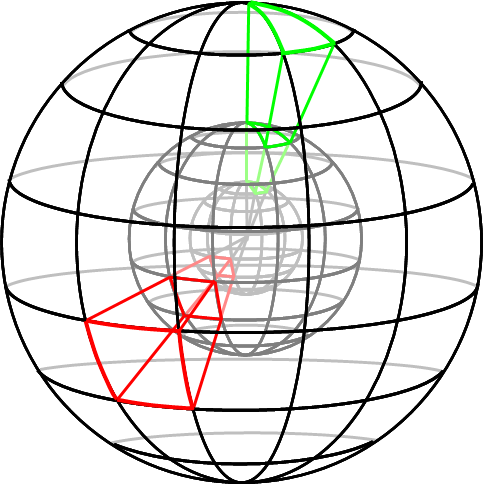
\includegraphics[width=0.24\textwidth]{images/3dsc}
    \label{fig:3dsc}
  }
  \subfloat[SHOT \cite{tombari2010unique}]{
    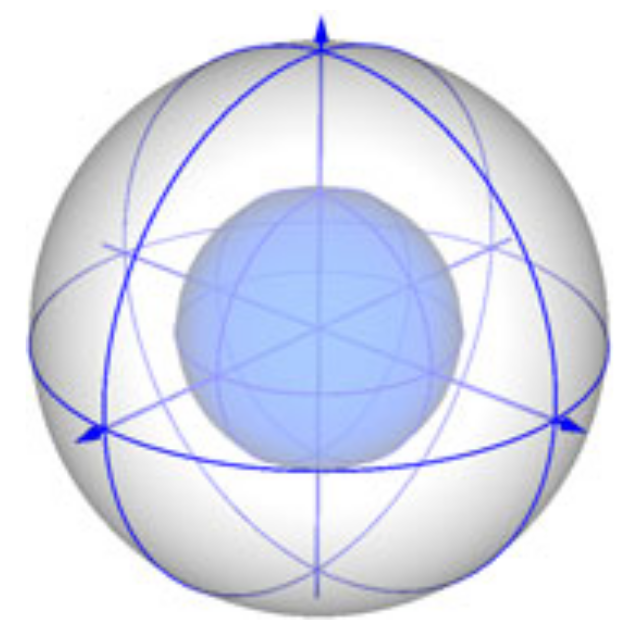
\includegraphics[width=0.24\textwidth]{images/shot}
    \label{fig:shot}
  }
  \subfloat[Context Shape \cite{shentu2008context}]{
    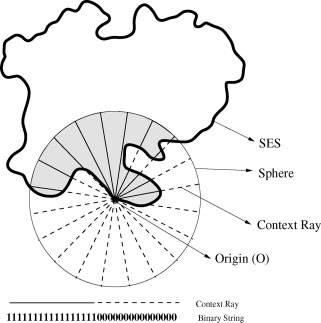
\includegraphics[width=0.24\textwidth]{images/contextshape}
    \label{fig:contextshape}
  }
  \subfloat[Integral Volume \cite{gelfand2005robust}]{
    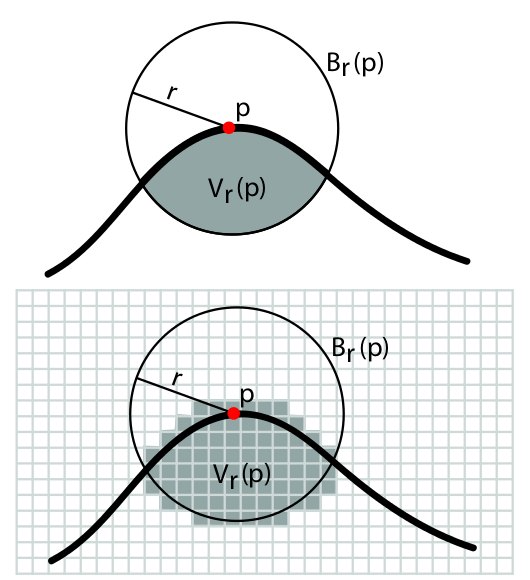
\includegraphics[width=0.24\textwidth]{images/volint}
    \label{fig:volint}
  }
  \caption{Visualisation of spherical descriptors.}
  \label{fig:descexample}
\end{figure}

3D Shape Context (3DSC) is an extension of the original Shape Context descriptor
for 2D images \cite{belongie2002shape}. A sphere is placed at a point, and its
``top'' is oriented to match the direction of the normal at the point. Bins are
created within the sphere by equally spaced boundaries in the azimuth and
elevation, and logarithmically spaced boundaries in the radial dimension (Figure~\ref{fig:3dsc}). The
logarithmic spacing means that shape distortions far from the basis point have
less effect on the descriptor. Each bin accumulates a weighted count based on
the volume of the bin and local point density \cite{frome2004recognizing}. 3DSC
does not compute a local reference frame --- the vector of the azimuth is chosen
randomly, and subdivisions computed from that. This means that a number of
descriptors equal to the number of azimuth divisions need to be computed and
stored in order to compensate, and the matching process is complicated as a
result. The Unique Shape Context (USC) solves this problem by defining a local
reference frame and using the directions of that reference frame to subdivide
the sphere \cite{tombari2010uniquesc}.

The Signature of Histograms of Orientations (SHOT) descriptor improves on 3DSC
by taking inspiration from SIFT and making extensive use of histograms. The
sphere is split into 32 volumes: 8 azimuth regions, 2 elevation and 2 radial
(Figure~\ref{fig:shot}). A local histogram is computed in each of the regions,
using the angle between the normal of points and the feature point. The local
histograms are then combined to form the final descriptor
\cite{tombari2010unique}. The authors also extend the descriptor to include
colour (COLORSHOT) \cite{tombari2011combined}.

The Rotation Invariant Feature Transform (RIFT) is a generalisation of SIFT. Using
intensity values computed at each point from the RGB values, a gradient is
computed. Concentric rings are placed around the initial point, and a histogram
of the gradient orientations is created for points within each ring. The
orientation of the gradient is computed relative to the line from the central
point so that the descriptor is rotation invariant. The descriptor is 2D --- one
dimension is the distance, the other the gradient angle. The distance between
two descriptors is measured using the Earth Mover's Distance (EMD), which is a
measure of the distance between two probability distributions
\cite{lazebnik2005sparse}.

Multi-scale descriptors are useful as they can be used to characterise regions
of varying size. Cipriano et al. introduce such a descriptor for use on meshes
\cite{cipriano2009multi}. It captures the statistics of the shape of the
neighbourhood of a vertex by fitting a quadratic surface to it. Vertices in the
region are weighted based on distance from an initial vertex, and a plane is
constructed using a weighted average of the face normals. The parameters of the
quadratic are then used to find its principle curvatures, which make up the
descriptor.

Work in protein-protein docking also uses 3D descriptors to help with
simulations of an otherwise lengthy and complex process. The Surface Histogram
is introduced by Gu et al. \cite{gu2012surface}, and uses the local geometry
around two points with specific normals on the surface of a protein. A
coordinate system is defined by the two points and the line between them, and a
rectangular voxel grid is defined around the points. The grid is then marked in
locations where the surface crosses the grid, and a 2D image is constructed by
squashing the data onto one of the axes. The descriptor is designed to
immediately give a potential pose for the docking.

Another example of a shape descriptor from biology is the Context Shape
\cite{shentu2008context}. A sphere is centred on a point, and rays are projected
from this point to points evenly distributed on the surface of the sphere (Figure~\ref{fig:contextshape}). Each
of the rays is divided into segments, with a binary value associated with each
segment depending on whether the segment is inside or outside the protein. To
compare the descriptor, a rotation is applied to match the rays, and a volume of
overlap is computed based on matching bits in the rays.
 
\begin{figure}
  \centering
  \subfloat[]{
    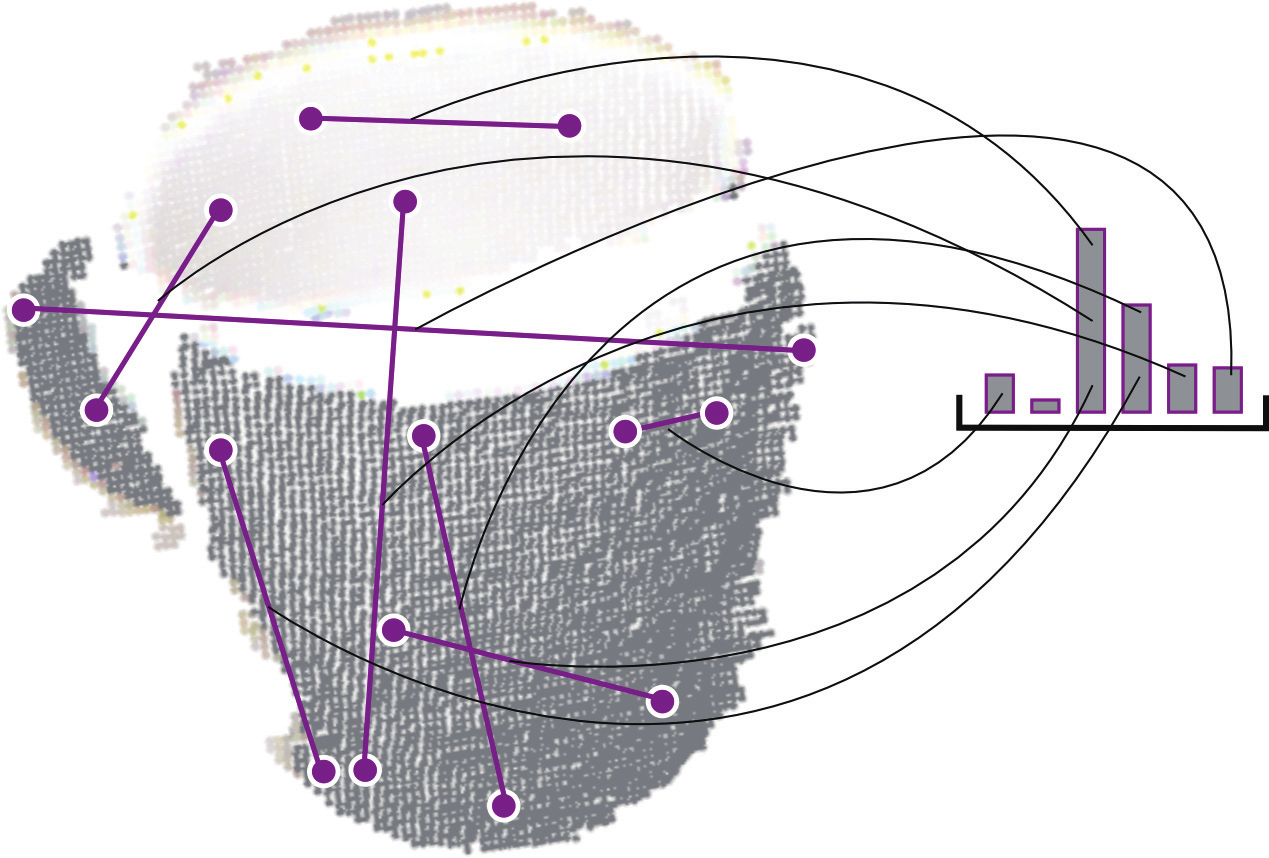
\includegraphics[width=0.23\textwidth]{images/wohl_d2}
  }
  \subfloat[]{
    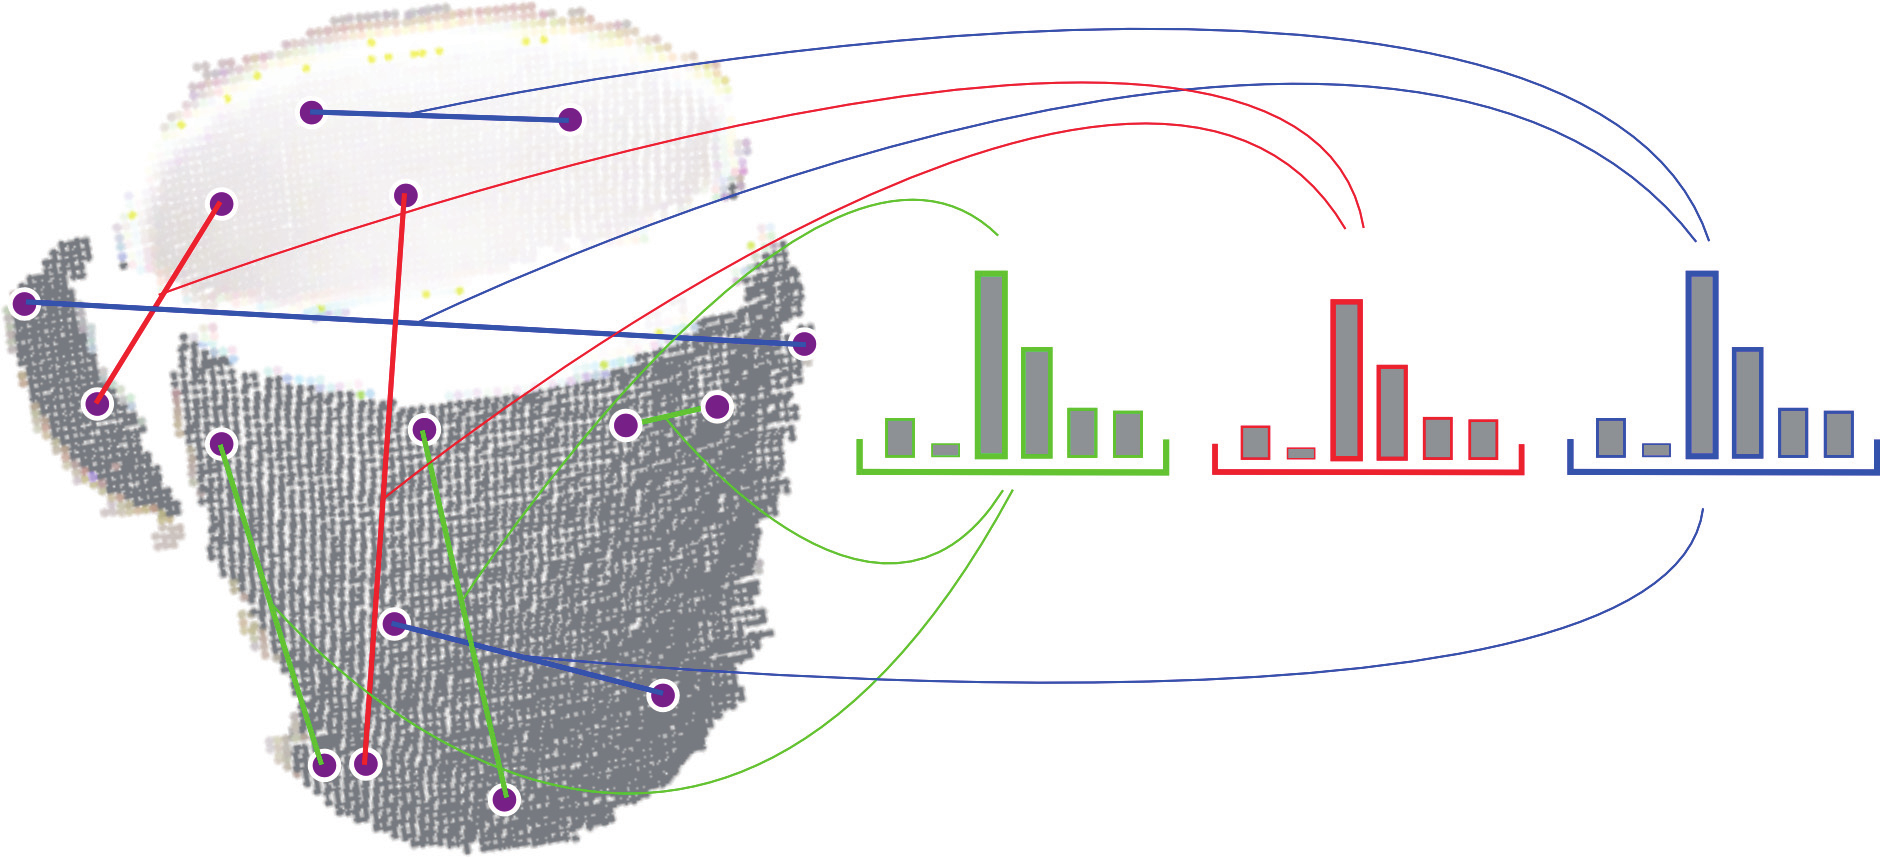
\includegraphics[width=0.23\textwidth]{images/wohl_onoff}
  }
  \subfloat[]{
    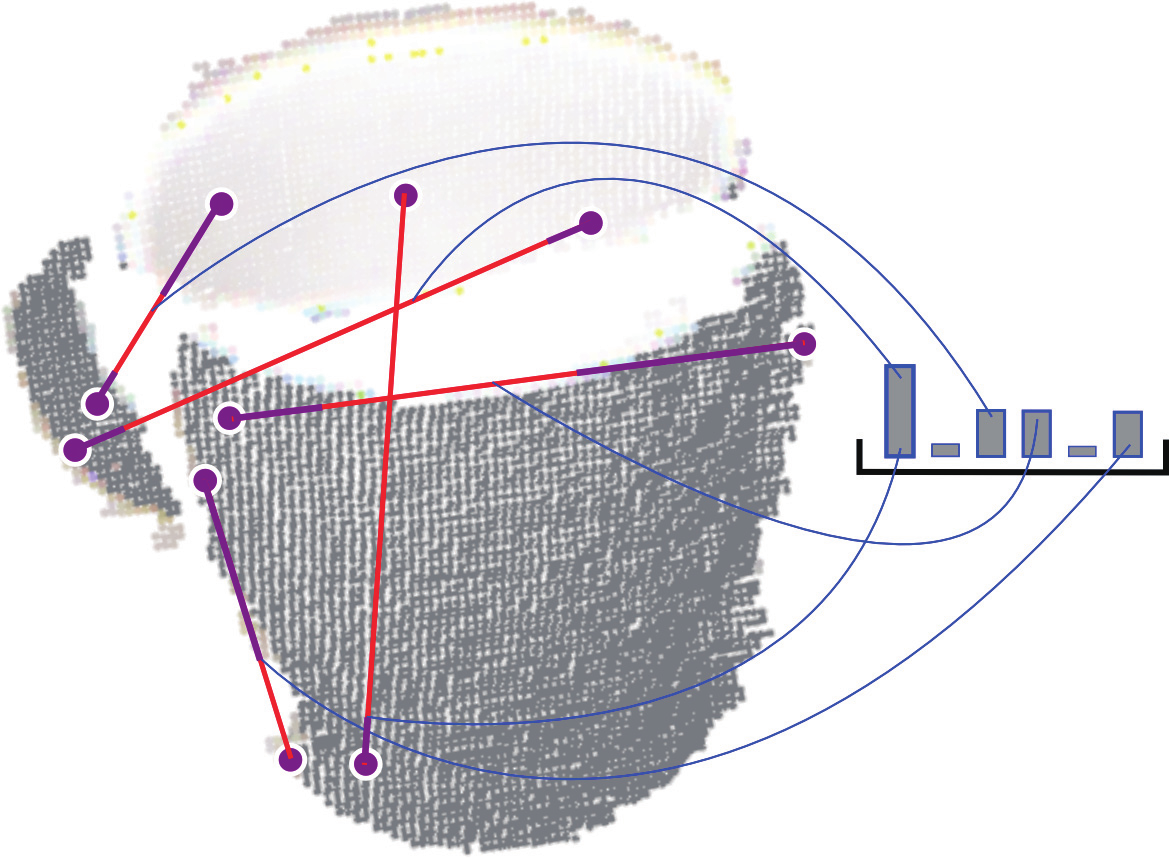
\includegraphics[width=0.23\textwidth]{images/wohl_ratio}
  }
  \subfloat[]{
    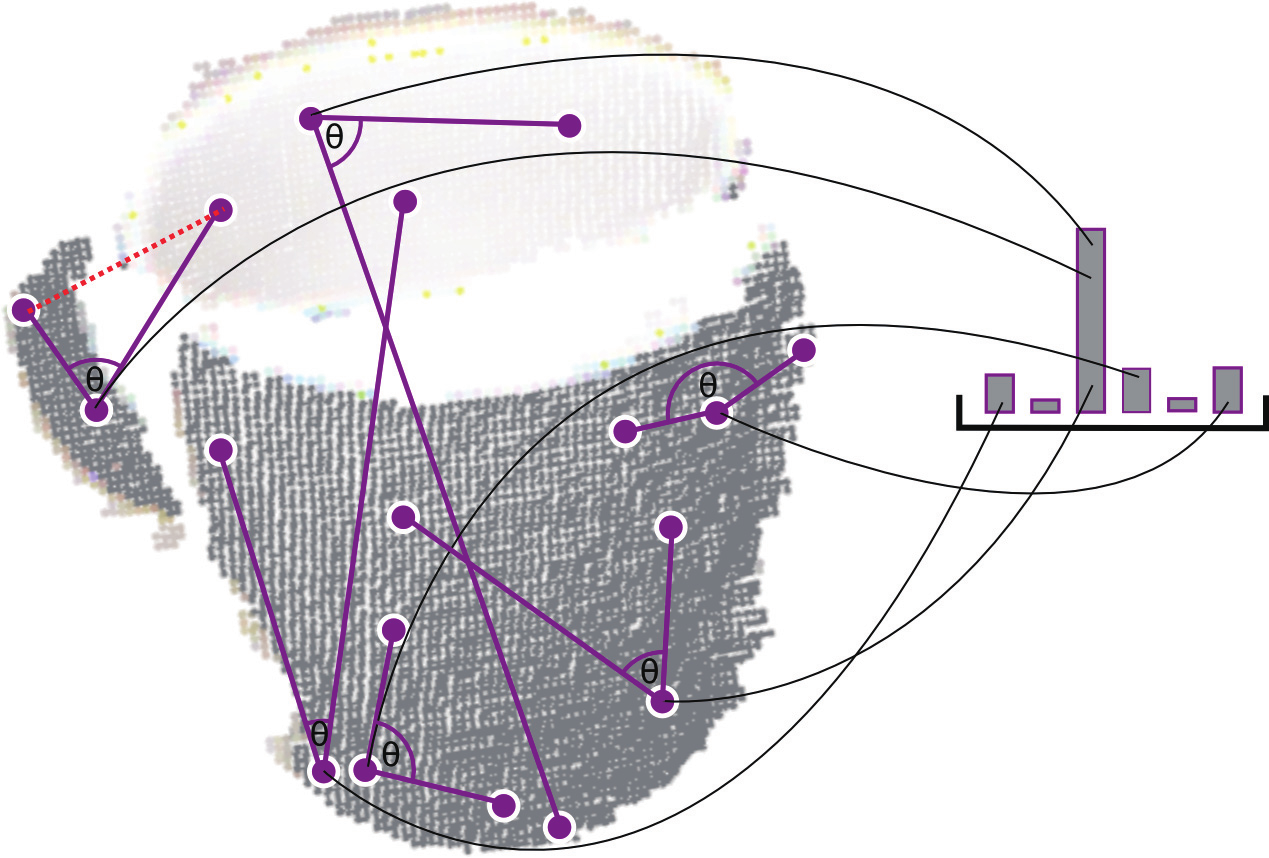
\includegraphics[width=0.23\textwidth]{images/wohl_a3}
  }
  \caption{Examples of the measures used to construct the Ensemble of Shape
    Functions histograms of \cite{wohlkinger2011ensemble}. a) Distance between
    points. b) Whether the points are on or off the model, or mixed. c) Ratio of
  line segments on and off the surface of the model. d) Angle between pairs of lines.}
  \label{fig:wohlESF}
\end{figure}

The splash descriptor was introduced by Stein et al. \cite{stein1992structural}.
A point on the surface with a given surface normal (the reference normal) is
chosen, and a slice around that with some geodesic radius (distance along the
surface) is computed. Points on the circle are selected using some angle step,
and the normal at that point is determined. A super splash is when this process
is repeated for several different radii. For each normal on the circle,
additional angles between it and a coordinate system centred on the reference
normal are computed. These angles and the angle around the circle are then
mapped into a 3D space, where polygonal approximation is made, connecting each
point with a straight line. Some additional computation is done to allow the
encoded polygons to act as a hash. Figure~\ref{fig:splash} shows part of the
formulation.

\begin{figure}
  \centering
  \subfloat[]{
    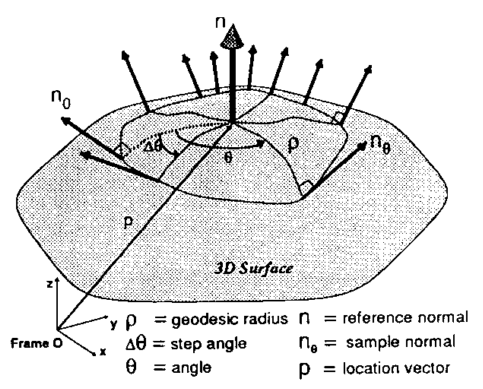
\includegraphics[width=0.32\textwidth]{images/splash}
  }
  \subfloat[]{
    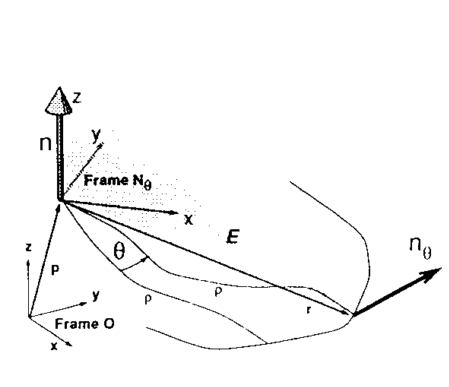
\includegraphics[width=0.32\textwidth]{images/splash_normals}
  }
  \subfloat[]{
    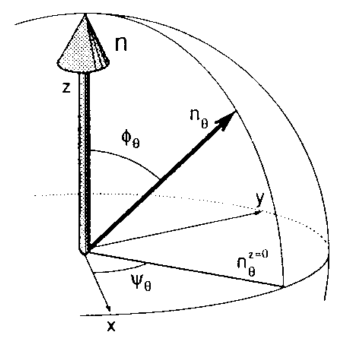
\includegraphics[width=0.32\textwidth]{images/splash_angles}
  }
  \caption{Splash descriptor \cite{stein1992structural}. a) shows the splash and
    normals around it. b) and c) show how the additional angles are defined.
  }
  \label{fig:splash}
\end{figure}

Point Signatures are similar to the splash descriptor in the sense that they
both sample points on a circle \cite{chua1997point}. This descriptor again
selects a reference normal, and has a specific radius. This time, the radius
defines a sphere around the point. The intersection of the surface with the
sphere is a 3D space curve. The orientation of the curve is defined by fitting a
plane to it. The distances between the space curve and the fitted plane at
sampled points define the signature of the reference point. These signatures can
be compared by lining them up and checking whether the query falls within the
tolerance band of previous signatures. Figure~\ref{fig:pointsig} shows
signatures from various surfaces.

\begin{figure}
  \centering
  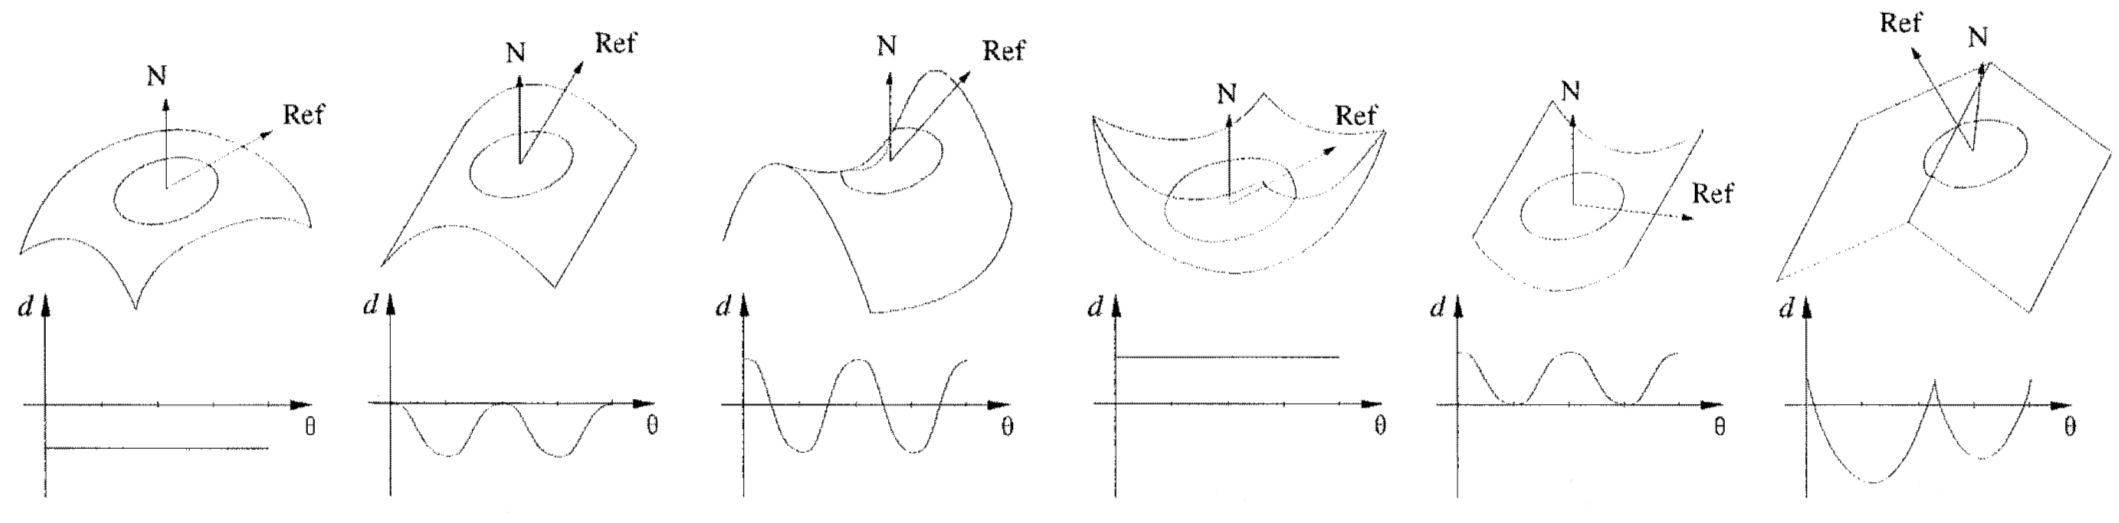
\includegraphics[width=\textwidth]{images/pointsig}
  \caption{Examples of the point signature responses to different surfaces
    \cite{chua1997point}. $d$ is the distance from the reference vector to the
    space curve defined by the intersection of the surface with a sphere centred
    at $N$. Ref rotates about $N$.}
  \label{fig:pointsig}
\end{figure}
\subsection{Combined Interest Point Extraction and Descriptors}
The Normal Aligned Radial Feature (NARF) is an interest point extraction method
with a feature descriptor. A score for the image points is determined based on
the surface changes at the point, and information about borders. An interest
value is computed from this based on the score of the surrounding points.
Smoothing is applied, and non-maximum suppression is applied to find the final
interest points. To compute the descriptor, rays are projected over the range
image from the centre at certain intervals. The intensities of cells lying under
the ray are weighted based on their distance from the centre, and a normalised
weighted average of the pairwise difference of cells is used to define each
element of the descriptor vector, which has a length equal to the number of rays
\cite{steder2011point}. The method is an improvement on a previous paper by the
authors \cite{steder2009robust}. A problem with this method is that it uses
range images directly. Point clouds can be used to generate range images by
looking at them from different viewpoints, but this adds complexity to the
method.

The integral volume descriptor is interesting as it combines interest point
selection and description into one. The descriptor is defined as the volume of
the intersection of a sphere centred at a point on the surface of an object with
the inside of the object (Figure~\ref{fig:volint}). Interest points are selected by histogramming the
descriptor values, identifying bins with a number of points less than a
specified values, and selecting points from these bins. To ensure features are
properly spaced, points in a certain radius of already selected points cannot be
used. By modifying the radius of the sphere used to generate the descriptor,
interest points at different scales can be selected \cite{gelfand2005robust}.

% \section{Point Matching}
% In \cite{chui2003new}, Chui and Rangarajan introduce an extension to ICP which
% allows for non-rigid registration and improved robustness to outliers. In
% contrast to ICP, their approach does not use the nearest-neighbour approach to
% define correspondence. Instead, they use an alternating algorithm similar to
% expectation maximisation. Annealing is used to prevent binary correspondences
% when the algorithm is not yet close to the solution --- at the beginning there
% is a large search range for correspondences, which gradually shrinks as the
% temperature decreases.

% \section{Model Matching}
% \begin{figure}
%   \centering
%   \subfloat[Conformal factors. High value indicates high required deformation to
%   sphere \cite{ben2008characterizing}.]{
%     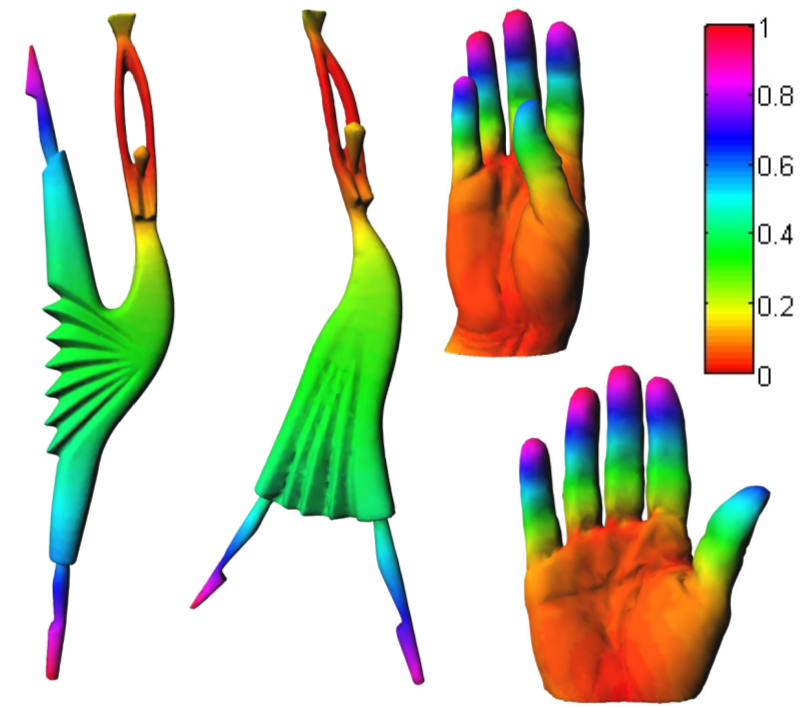
\includegraphics[width=0.48\textwidth]{images/conformal.png}
%     \label{fig:conform}
%   }
%   \caption{Model matching approaches}
%   \label{fig:modelmatch}
% \end{figure}
% In \cite{ben2008characterizing}, Chen et al. describe another approach to model
% matching using conformal factors. This technique uses ideas from conformal
% geometry, transforming the mesh of an object such that it has a uniform Gaussian
% curvature. Information is stored about how much deformation is needed locally to
% globally transform the object into a sphere --- this is the conformal factor.
% The factor is based on a global computation on the whole mesh, as opposed to
% per-vertex computations of the Gaussian curvature, which makes it much smoother
% and appropriate for use in histograms. The histogram of a sample of the factors
% is used as a descriptor, and is pose invariant, as seen in
% Figure~\ref{fig:conform}. The authors say that it should be possible to use the
% approach in partial model matching.
\section{Storing and Querying Descriptors}
There are several techniques for storing and querying descriptors, mostly based
on some form of tree. Recently, the k-d tree\cite{bentley1975multidimensional,
  friedman1977algorithm} has been used for efficient approximate matching with
either an error bound \cite{arya1998optimal}, where there is a bound placed on
the error between the true nearest neighbour and the one found, or a time bound
\cite{beis1997shape}, where the search is stopped after examining a certain
number of leaf nodes. Further improvements on the k-d tree are introduced in
\cite{silpa2008optimised}, where multiple randomised trees are used to optimise
the search. A priority search tree algorithm is introduced in
\cite{muja2014scalable}, which appears to be very effective. This may be the
same one as in \cite{muja2009fast}. The algorithm in the last two papers has
been integrated into PCL, which is useful.

A different approach to nearest neighbour search is the balltree, which uses
hyperspheres in a hierarchy to enclose points in the space
\cite{omohundro1989five}. Unlike the k-d tree, regions on the same level of the
tree are allowed to intersect, and do not need to partition the whole space,
which gives the balltree its representative power.

The vocabulary tree \cite{nister2006scalable} makes use of techniques from
document search to index images. Using $k$-means clustering, construction stage
creates a hierarchical quantisation of the image patch descriptors. In the query
phase, descriptors are compared to the cluster centres, and go down the tree
until a leaf is reached. The path through the tree is used as a scoring measure
to present retrieval results.

Philbin et al. \cite{philbin2007object} show that flat (single-level) $k$-means
clustering can be scaled to large vocabulary sizes if approximate nearest
neighbour methods are used. Early systems for image retrieval used a flat
clustering scheme, which could not scale to large vocabularies
\cite{sivic2003video}. The paper also introduces a re-ranking method which uses
spatial correspondences, which improves the retrieval quality.

Boiman et al. \cite{boiman2008defense} introduce the Naive Bayes Nearest
Neighbour (NBNN) classifier. It uses nearest neighbour distances in the space of
descriptors instead of images, computing ``image-to-class'' distances without
quantising the descriptors. In general, quantisation allows for dimensionality
reduction, at the expense of the discriminative power of descriptors. NBNN ``can
exploit the discriminative power of both (few) high and (many) low informative
descriptors''. The problem here is that the classes must be known beforehand,
and in our case we do not have that information. The local NBNN
\cite{mccann2012local} does not do the search based on classes. Instead, all the
descriptors are merged into a k-d tree on which approximate $k$-NN is run to
find descriptors in the local region of a query descriptor. A distance to
classes not present in the $k$-NN region is approximated by the distance to the
$k+1$th neighbour.

% \begin{figure}
%   \centering
%   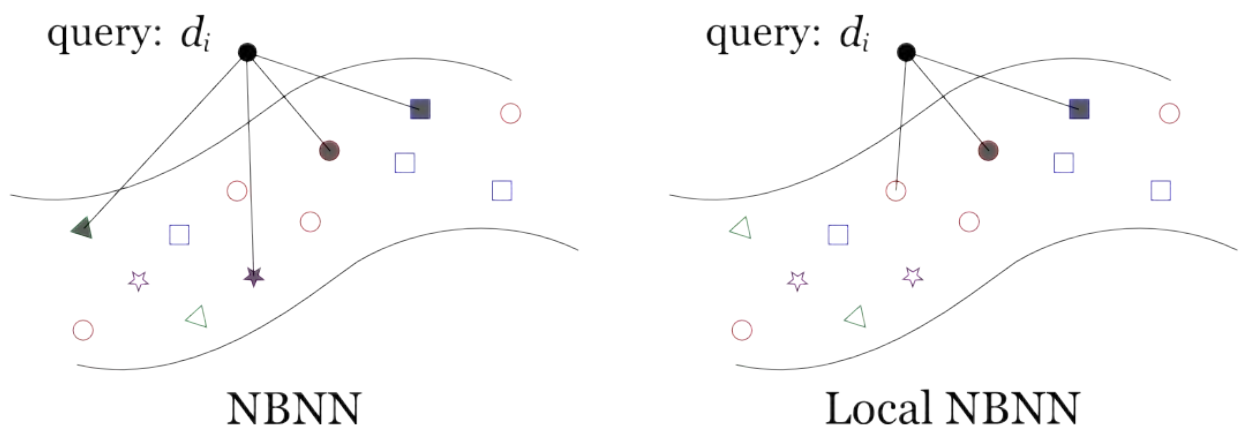
\includegraphics[width=0.6\textwidth]{images/nbnn_comp}
%   \caption{NBNN vs. local NBNN \cite{mccann2012local}. NBNN looks at the nearest
%   neighbours in all classes, whereas local NBNN just looks at the local region,
%   regardless of what classes are present in the database.}
%   \label{fig:nbnncomp}
% \end{figure}

Funkhouser and Shilane present a method for querying a database of 3D objects
represented by local shape features \cite{funkhouser2006partial}. Partial
matches (correspondences) are stored in a priority queue sorted by geometric
deformation and the feature similarity. This means that only objects in the
database with a high probability of being a match need to be processed.

Some work has been done on optimising the retrieval of relevant images by
learning from user input \cite{rui2000optimizing}. When retrieved images are
presented, the user ranks them in terms of relevance, and this rank is then used
to improve the relevance of future searches.

\section{Other}
Here are some papers which are interesting and might yield some interesting
insights or techniques, but do not directly relate to our problem for whatever
reason.

The convolutional k-means descriptor introduced in \cite{blum2012learned} and
BRAND descriptor \cite{nascimento2012brand} work on RGB-D images, not directly
on point clouds. \cite{kim20113d} makes use of the visibility of objects and
point pair features to improve recognition performance. Kim et al. use the RGB
image and corresponding point cloud to improve the hypotheses for segmentation
\cite{kim2013accurate}. \cite{mueller2013recognition} uses a growing neural gas
to characterise the shape of parts of objects.

\chapter{System Development}
\label{chap:devel}
Talk about how different parts of the system were developed, why they are
required, what benefits they provide, how they work, and so on.
\section{Preprocessing}
Basic description of what segmentation is, discussion about whether or not it is
necessary
\subsection{Room Rotation and Trimming}
How the data is gathered, what is done to it at the beginning to remove some points
\subsection{Normal Extraction}
Normal and plane extraction section order depends partly on the order in which
it is done. Talk about how normal extraction can help with plane extraction, if
I do that.
\subsection{Plane Extraction}
Basic description of RANSAC or whichever of its extensions I end up using.
\section{Feature Extraction}
Talk specifically about each of the features used and their good/bad points, and
how the features extraction is done (not particularly complex, probably)
\section{Object Query}
Query methods, how the database and query object are compared.

\chapter{Implementation}
\label{chap:impl}
Description of any parts of the implementation which are non standard or worth a
mention. Perhaps talk about PCL and version control, as well as documentation
and some other general software approaches to the system?
\chapter{Experimental Results}
\label{chap:exp}
Description of experiments and experimental results with different
configurations of the system.
\section{Segmentation}
Apply different segmentation methods/parts of the segmentation method, and see
how they affect the overall system performance, as well as the time taken to
complete the segmentation.
\section{Feature Extraction}
Same as above, but for feature extraction. Try different features and see which
give best performance. Consider normal extraction cost for those features which
require it.
\section{Object Query}
This is evaluated in the previous two sections, but maybe there is more than one
method of finding the query object. Multi-index tree vs single index tree, for
example.
\chapter{Conclusion and Further Work}
\label{chap:conc}
Describe what the project was about, what was achieved, summarise the
experiments, describe what can be improved.


%\printbibliography
\end{document}